Use case scenarios of the approximation technique we discuss have their own constraints and limitations.
For instance, approximation requirements should have precisely specified exponent $j$ in $X^j$ because
for each $j$ there is a matching polynomial $P(m,X,N)$.
Perfectly, there should be a set precompiled polynomials $P(m,X,N)$ matching precise exponent $j$ in $X^j$ over
precisely defined approximation range with required error of approximation $E$ as a constraint.
Generally, the approximation of power function $X^j$ by $P(m,X,N)$ can be broken down into the following steps
\begin{enumerate}
    \item Define the exponent $j$ in $X^j$
    \item Define the required error threshold $E$
    \item Define the required interval of approximation $I$
    \item Choose and precompile polynomials $P(m,X,N)$
    so that the required interval of approximation and error threshold $E$ are satisfied
    \item Define a set of knots so that the error threshold $E$ and the interval of approximation $I$ requirements are satisfied
\end{enumerate}
Defining set of spline knots essentially requires an inspection of the
convergence intervals between $X^j$ and $P(m,X,N+t_k)$
by choosing knots such that the interval of approximation and error threshold are satisfied.
Consider an example.
Let be the following approximation requirements
\begin{enumerate}
    \item Exponent $j=3$
    \item Percentage error threshold $E\leq 1\%$
    \item Interval of approximation $10 \leq X \leq 15$
\end{enumerate}
Now we have to choose a set of polynomials $P(m, X, N+t_k)$ based on which we adjust a set of spline knots.
We can safely choose integers $t_k$ in range $10 \leq t_k \leq 15$ because
of the following properties of $P(m,X, N)$.
\begin{align*}
    P(m,X, X) &= X^{2m+1} \\
    P(m,X, X+1) &= (X+1)^{2m+1} - 1
\end{align*}
Therefore, for each two consequential points $N=X, N=X+1$ the absolute difference is 1, making that range
at least $1\%$ percentage error for $X^j \leq 100$.
I have chosen the approximation range $10 \leq X \leq 15$ and $j=3$ intentionally to show the spline approximation with
percentage error threshold less than $1\%$.
Therefore, to approximate $X^3$ in the range $10 \leq X \leq 15$, we use the following spline function
\begin{align}
    X^3 \approx
    \begin{cases}
        P(1,X,10) = -2300 + 330X, & 10 \leq X < 11 \\
        P(1,X,11) = -3025 + 396X, & 11 \leq X < 12 \\
        P(1,X,12) = -3888 + 468X, & 12 \leq X < 13 \\
        P(1,X,13) = -4901 + 546X, & 13 \leq X < 14 \\
        P(1,X,14) = -6076 + 630X, & 14 \leq X \leq 15
    \end{cases}
    \label{eq:spline_approximation_of_cubes}
\end{align}
Graphically, this linear approximation of cubes looks as follows
\begin{figure}[H]
    \centering
    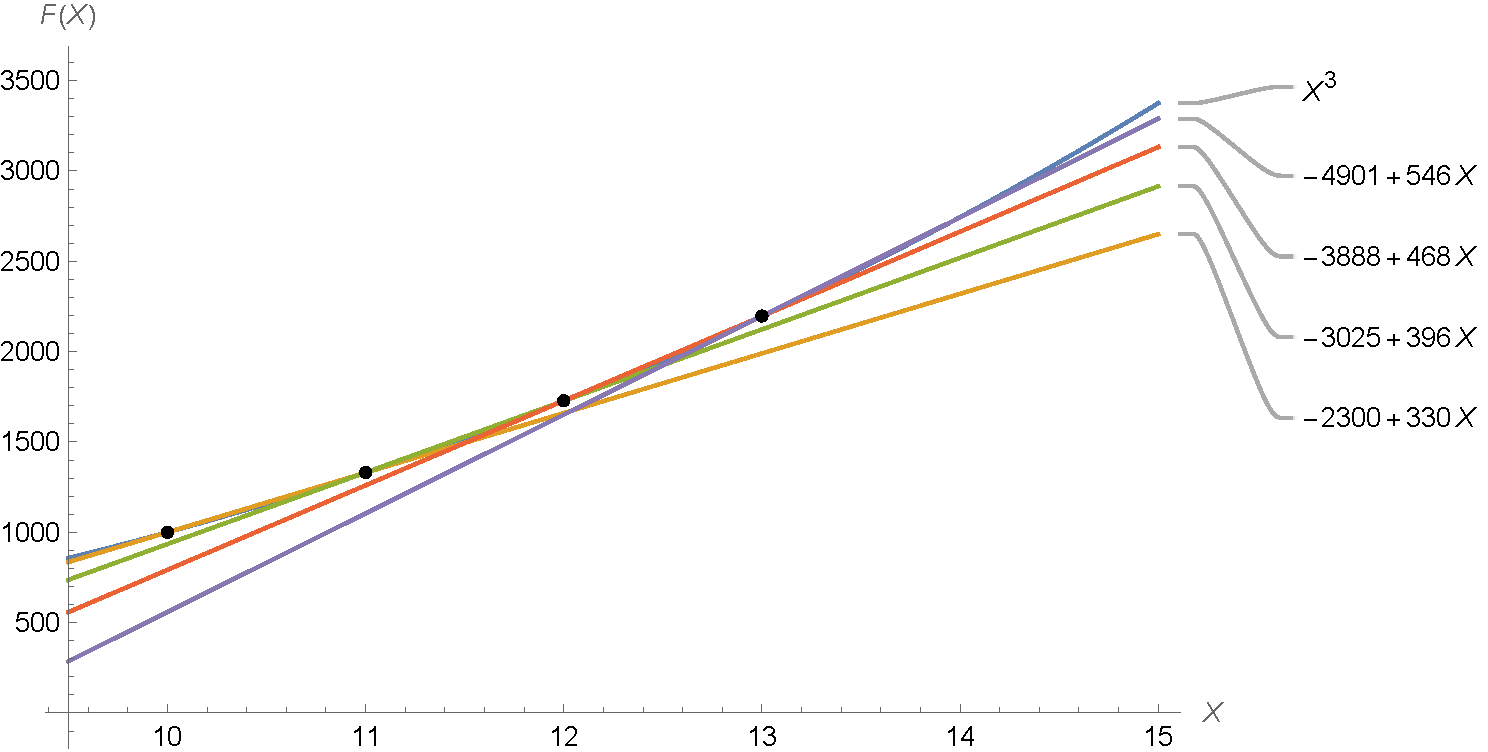
\includegraphics[width=1\textwidth]{sections/images/08_plots_of_cubes_power_with_p_2_10_15}
    ~\caption{
        Approximation of cubes $X^3$ by splines~\eqref{eq:spline_approximation_of_cubes}.
        Convergence interval is $10 \leq X \leq 15$ with percentage error $E\leq 1\%$.
    }
    \label{fig:08_plots_of_cubes_power_with_p_2_10_15}
\end{figure}
where the spline knots are integers in the range $10 \leq N \leq 14$.

The same principle applies for even exponent $j=4$ in $X^j$ with the same convergence interval $10 \leq X \leq 15$
and approximation error under $1\%$ constraints
\begin{align}
    X^4 \approx
    \begin{cases}
        P(1,X,10) \cdot X = -2300X + 330X^2, & 10 \leq X < 11 \\
        P(1,X,10) \cdot X = -3025X + 396X^2, & 11 \leq X < 12 \\
        P(1,X,10) \cdot X = -3888X + 468X^2, & 12 \leq X < 13 \\
        P(1,X,10) \cdot X = -4901X + 546X^2, & 13 \leq X < 14 \\
        P(1,X,10) \cdot X = -6076X + 630X^2, & 14 \leq X \leq 15
    \end{cases}
    \label{eq:spline_approximation_fourth_power}
\end{align}
Which graphically looks as follows
\begin{figure}[H]
    \centering
    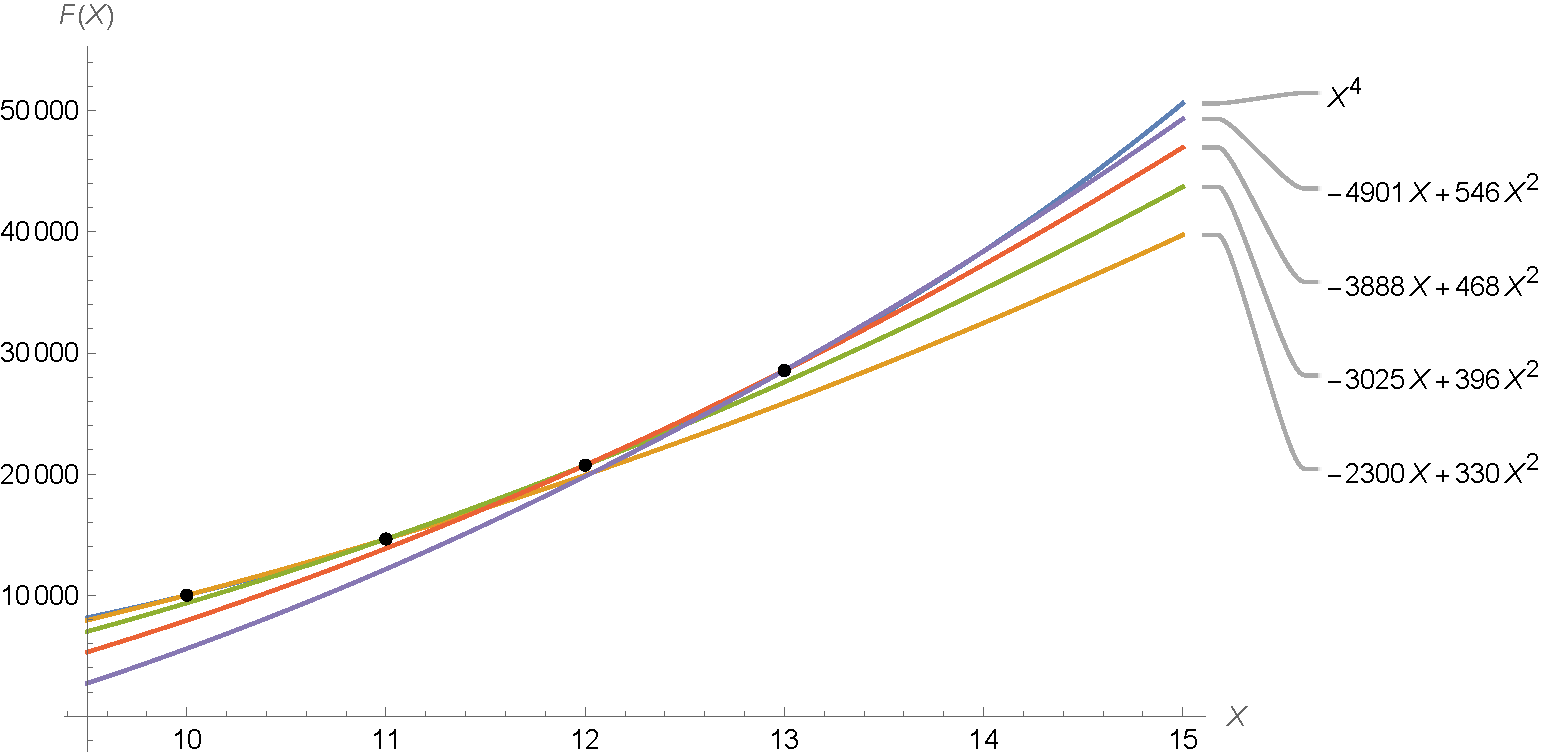
\includegraphics[width=1\textwidth]{sections/images/09_plots_of_fourth_power_with_p_2_10_15_times_x}
    ~\caption{
        Approximation of $X^4$ by splines~\eqref{eq:spline_approximation_fourth_power}.
        Convergence interval is $10 \leq X \leq 15$ with percentage error $E\leq 1\%$.
    }
    \label{fig:09_plots_of_fourth_power_with_p_2_10_15_times_x}
\end{figure}
In general, for each variation of $X^j$ such that $X^j \geq 100$ the approximation can be done using
splines in $P(m,X, N)$ over the interval $A \leq X \leq B$ with spline knot vector be the integers in
range from $A$ to $B$ so that knots vector is $\{A, A+1, A+2, \ldots, B \}$.
Because,
\begin{align*}
    P(m,X, X) &= X^{2m+1} \\
    P(m,X, X+1) &= (X+1)^{2m+1} - 1
\end{align*}
This can be further optimized depending on the value of $N$ in $P(m,X,N)$ because the convergence interval
with the power function $X^j$ increases as $N$ grows.
